% !TeX spellcheck = de_DE
\section{Finanzierung - Business Angels und Venture Capital}
\subsection{Bootstrapper vs. Funder}
\begin{itemize}
	\item \textbf{Bootstrapper:} Benutzen eigenes Geld, Privatvermögen oder Geld von Kunden. Funktioniert oft nur wenn schnell ein Produkt da ist.
	\item \textbf{Funder:} Externe Kapitalgeber
\end{itemize}

\subsection{Unternehmensfinanzierung}
\begin{itemize}
	\item Unternehmen müssen jederzeit zahlungsfähig sein
	\item Die meisten (Start-up) Konkurse sind auf Finanzierungs- bzw. Liquiditätsprobleme zurückzuführen.
	\item Gewinn und Rentabilität sind die „Nahrung“ des Unternehmens, die Liquidität ist der „Sauerstoff“. Gewinn ist das langfristige Ziel.
	\item Eine fundierte Finanzplanung (1 – 5 Jahre) sowie eine aktuelle und verlässliche Liquiditätsplanung (3 – 12 Monate) sind ein Muss.
	\item Für jedes Projekt muss eine optimale Finanzierung individuell gefunden werden.
	\item Es gibt unterschiedliche Finanzierungsquellen mit verschiedenen Eigenschaften.
\end{itemize}

\subsubsection{Finanzierungsphasen}
\begin{multicols}{2}
	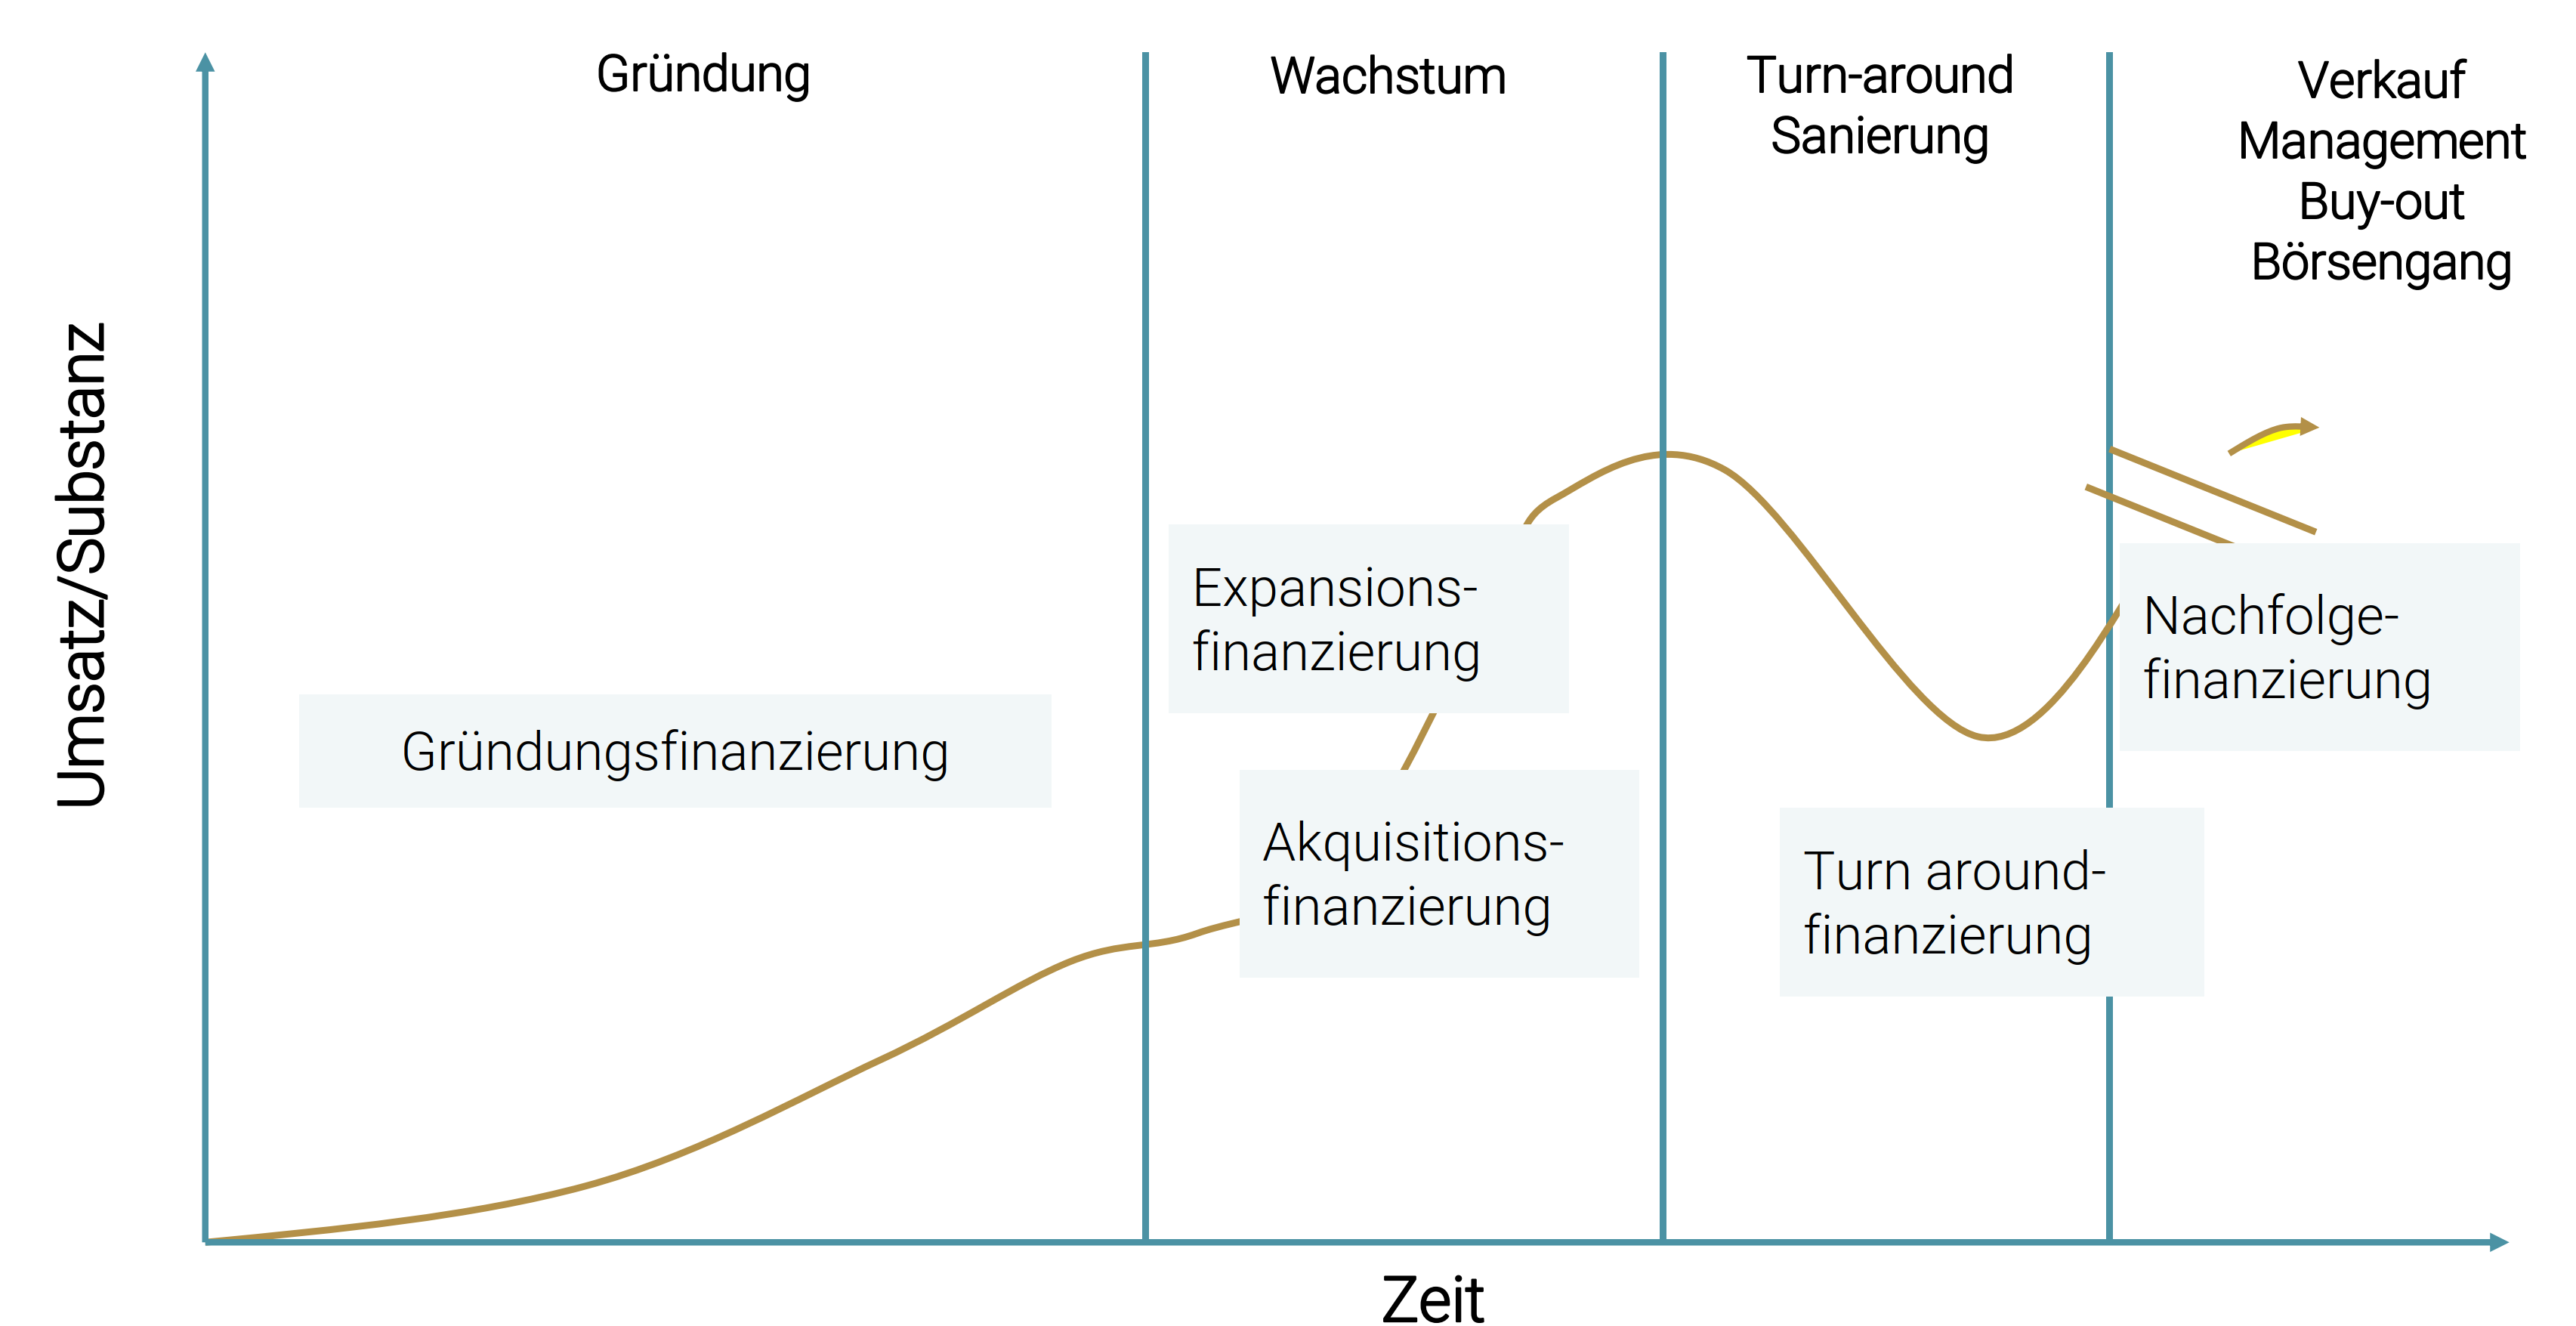
\includegraphics[width=1\linewidth]{images/finanzierungsphasen}
	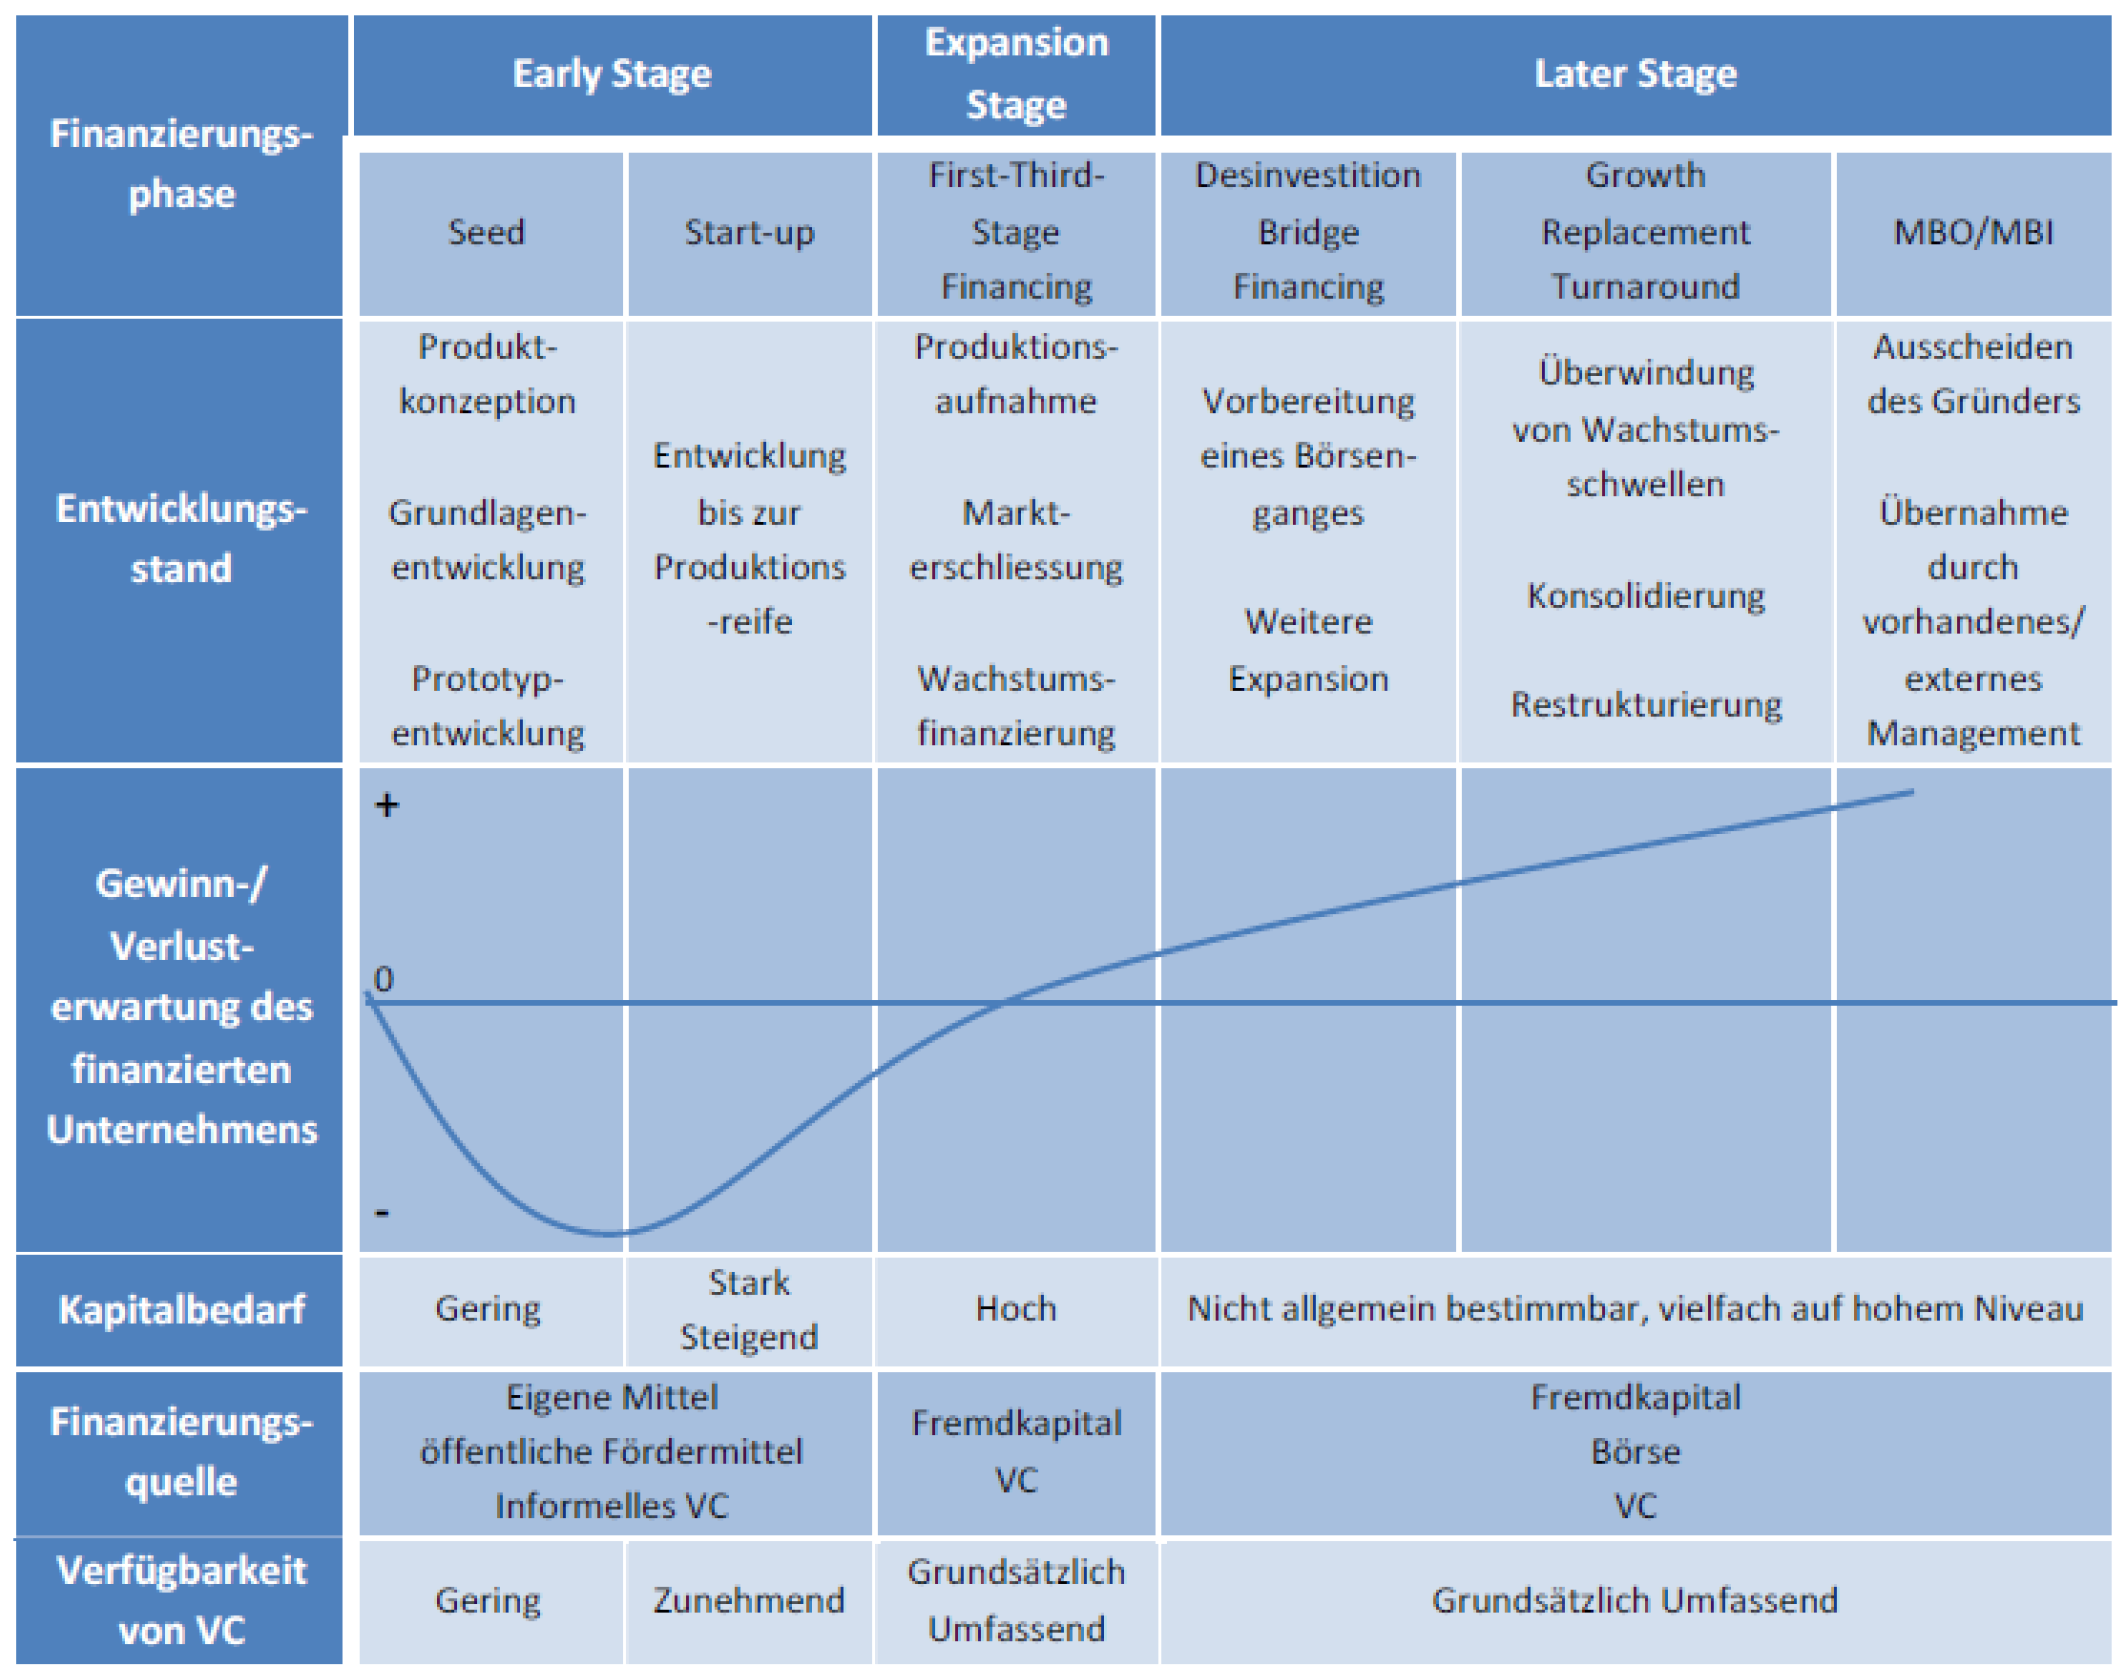
\includegraphics[width=1\linewidth]{images/finanzierungsphasen_2}
\end{multicols}

\subsubsection{Finanzierungsformen}
\begin{multicols}{2}
	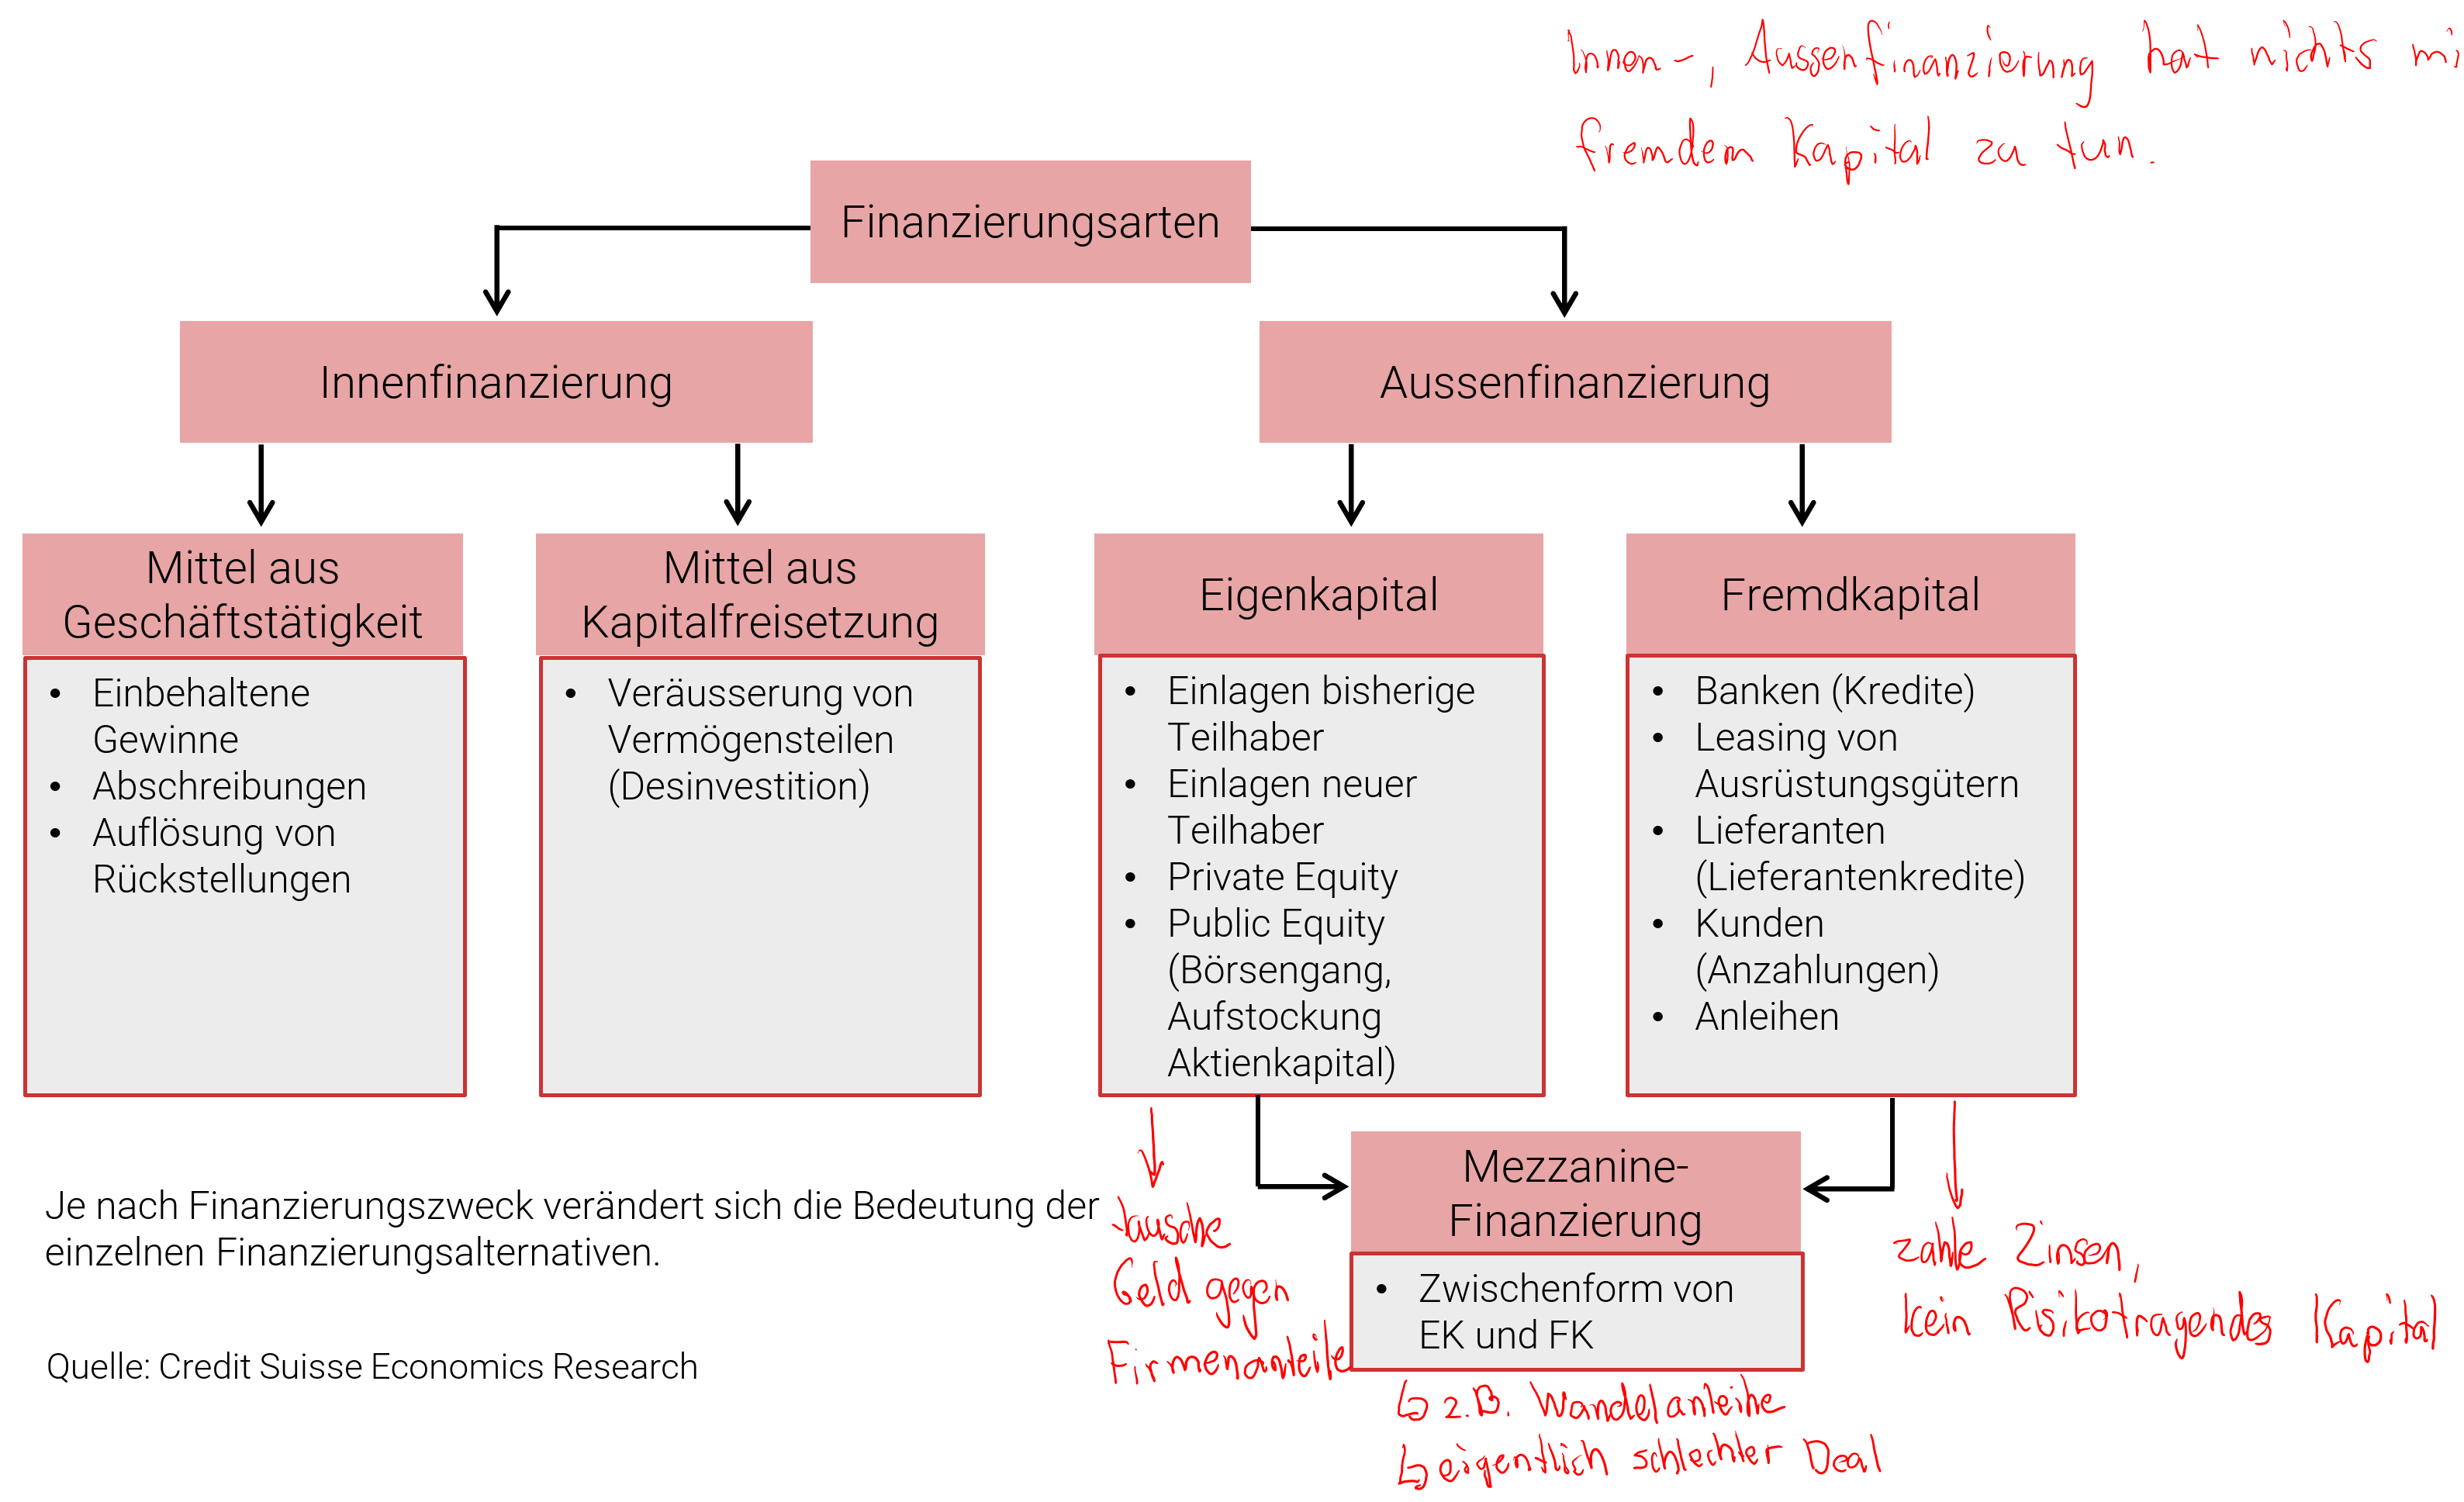
\includegraphics[width=1\linewidth]{images/finanzierungsformen}
	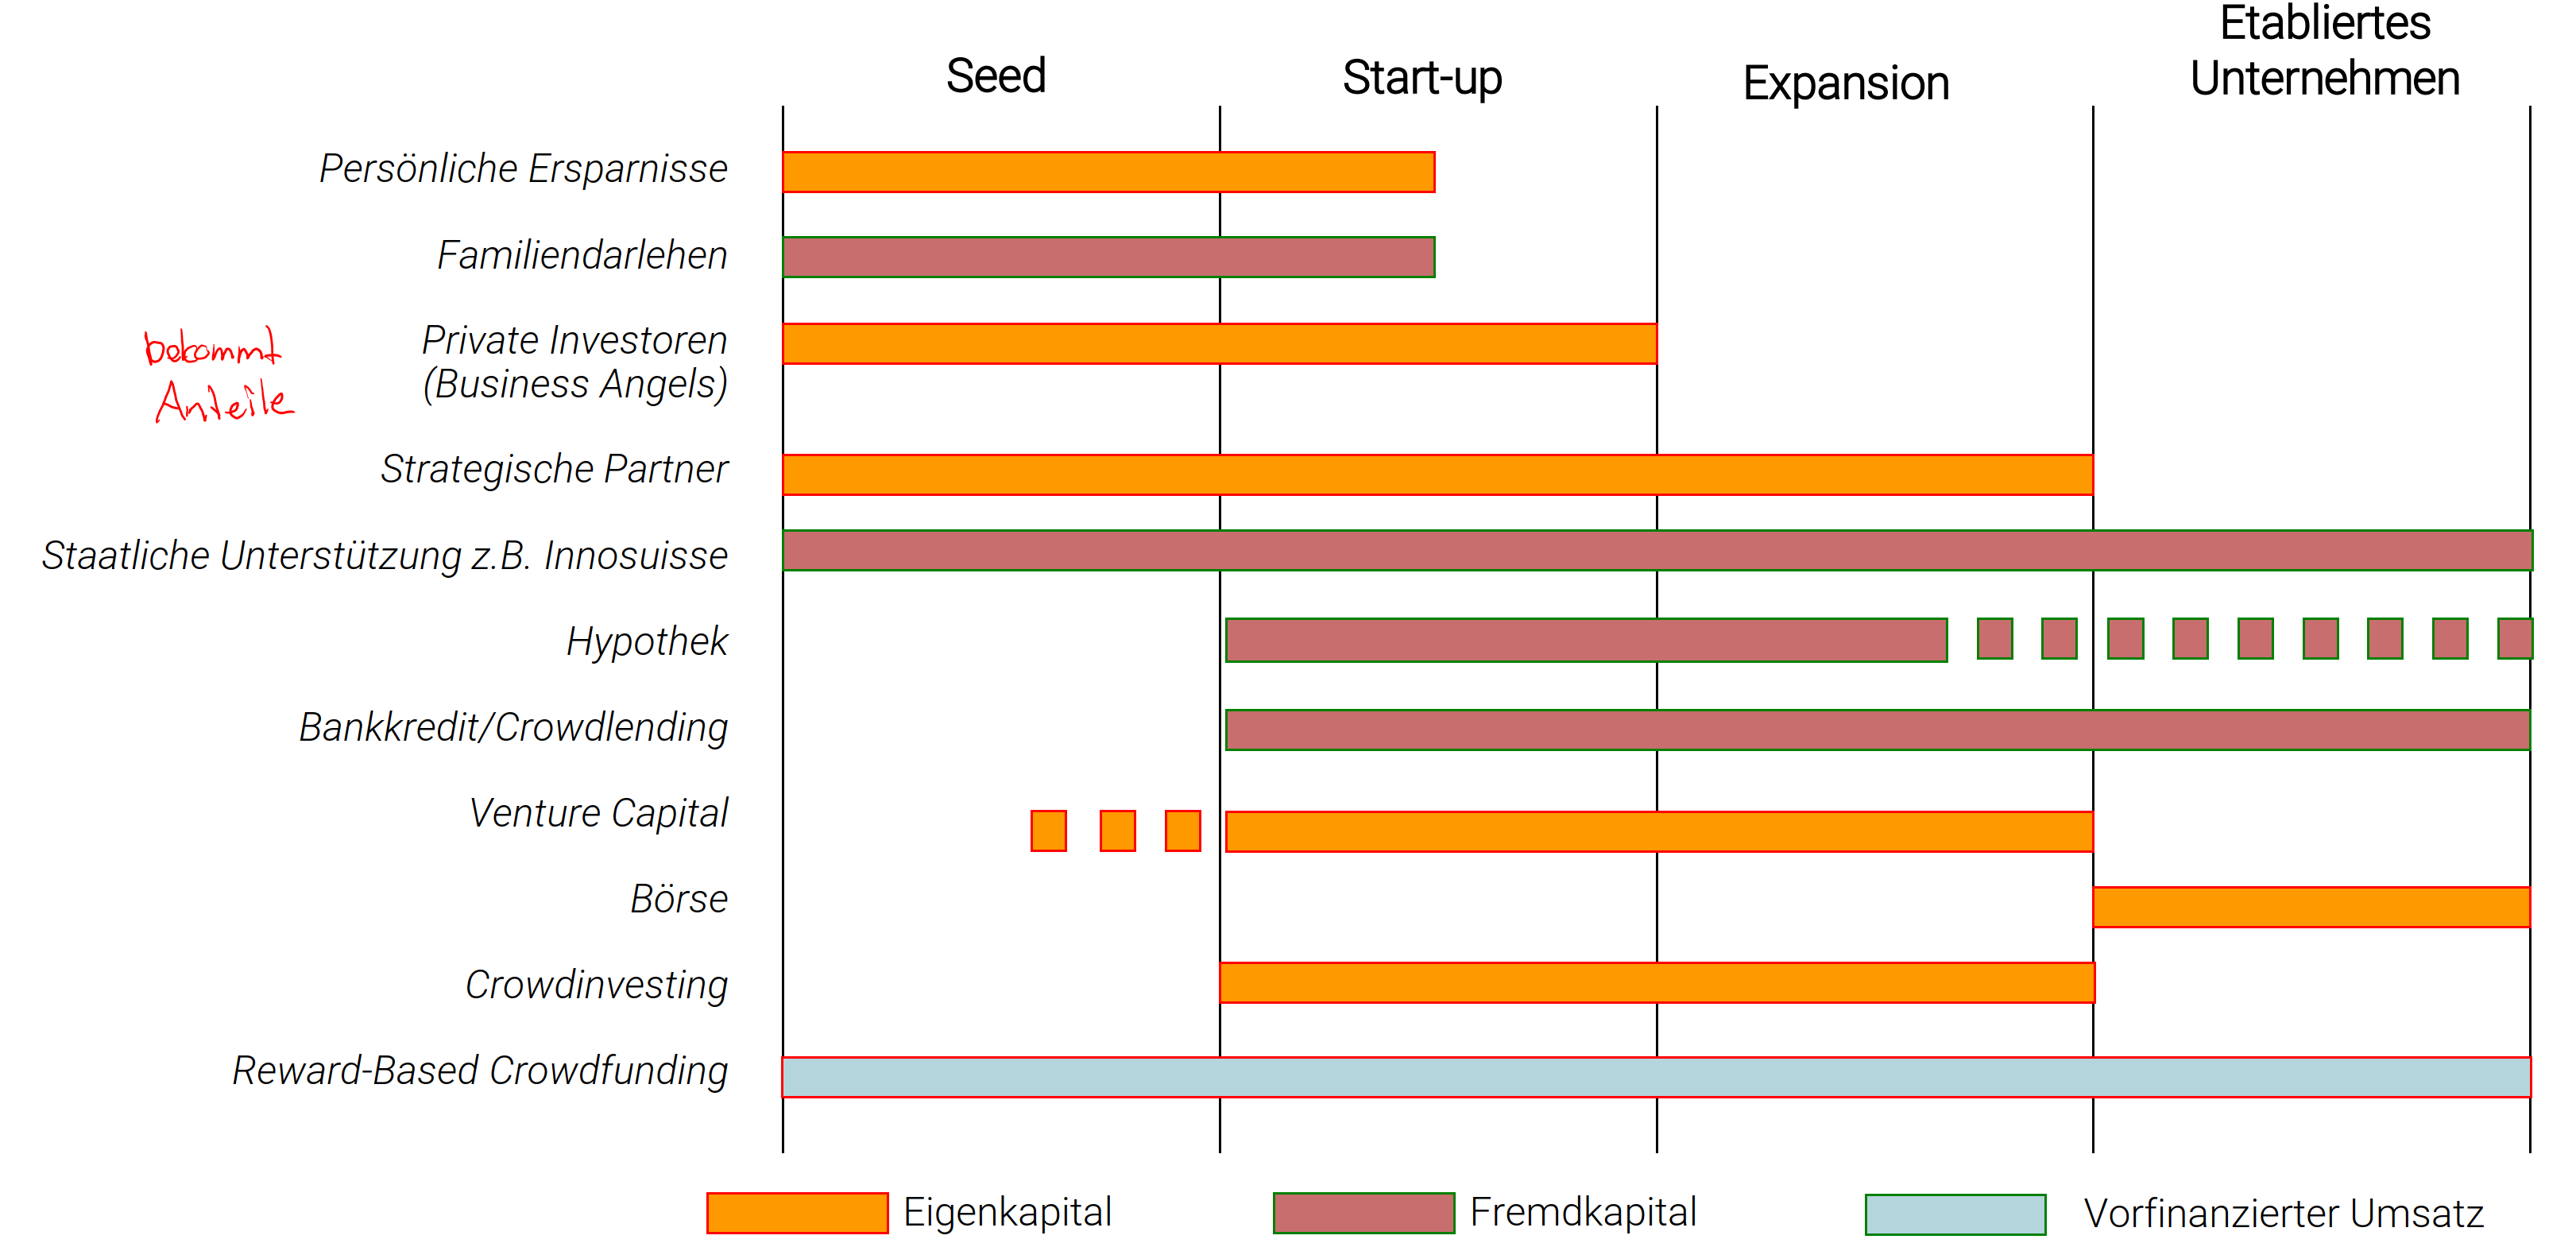
\includegraphics[width=1\linewidth]{images/finanzierungsformen_2}
\end{multicols}

\textbf{Alternative Finanzierungsformen:}
\begin{itemize}
	\item Business Angels
	\item Venture Capital
	\item Corporate Venture Capital
	\item Fremd- oder Eigenkapital von Verwandten und Freunden
	\item Crowdfunding
	\item Crowdinvesting
	\item Crowdlending
	\item Finanzhilfen durch staatliche Wirtschaftsförderung (z.B. Innosuisse)
	\item Bürgschaften durch Bürgschaftsgenossenschaften (keine direkte Finanzierung, sondern Sicherheit für Bankkredite)
\end{itemize}

\subsubsection{Finanzierungsmöglichkeiten}
Abgesehen von Höhe des Finanzbedarfs, stellen sich bei der Finanzierung folgende Fragen:
\begin{itemize}
	\item Wofür soll das Kapital investiert werden (Verwendungszweck)?
	\item Für welche Zeitdauer soll das Kapital beschafft werden?
	\item Wie lautet das Angebot (Deal) an potenzielle Kapitalgeber?
	\item Welche Rendite können die Investoren erwarten?
	\item Aus welchen Quellen soll die Finanzierung erfolgen (Mittelherkunft)?
\end{itemize}

\subsection{Venture Capital}
Merkmale der Venture Capital Finanzierung sind:
\begin{itemize}
	\item Beteiligungen statt Darlehen (Eigenkapital)
	\item Genaue Prüfung
	\item Aktive Unterstützung der Unternehmensentwicklung (Management-Unterstützung)
	\item Vertragliche Vereinbarung der Zusammenarbeit
	\item Ausstiegsregelung
\end{itemize}
VC = Finanzierungsform für Jungunternehmen (Start-ups) mit sehr hohem Risikoprofil und dadurch auch hohe Renditechancen

\subsubsection{Exit Möglichkeiten}
\begin{tabular}{|p{0.15\linewidth}|p{0.25\linewidth}|p{0.5\linewidth}|}
	\hline 
	\textbf{Alternativen der Desinvestition} & \textbf{Charakteristika} & \textbf{Ausgewählte Vor- und Nachteile} \\ \hline
	Buy Back & Im Regelfall Verkauf	an Altgesellschafter & \begin{itemize} 
																\item[+] Erhalt der Unternehmenskultur
																\item[-] Übernahme eines hohen finanziellen Risikos
																\item[-] Kein strategischer Nutzen aus Transaktion
															\end{itemize} \\ \hline
	Trade Sale & Veräußerung an	einen industriellen	Investor & \begin{itemize} 
																	\item[+] Schnelle / kostengünstige Abwicklung
																	\item[+] Nutzung von Synergiepotentialen
																	\item[-] Aufgabe der Unternehmenskontrolle
																\end{itemize} \\ \hline
	Secondary Purchase & Verkauf an einen Finanzinvestor & \begin{itemize} 
																\item[+] Nutzung der Branchenerfahrung des Finanzinvestors
																\item[-] Einräumung eines Mitspracherechts an den Finanzinvestor bei strategischen Entscheidungen
															\end{itemize} \\ \hline
	Börsengang & Einführung der Gesellschaft am Kapitalmarkt & \begin{itemize} 
																	\item[+] Chance auf einen höheren Verkaufserlös im Vergleich zum Trade Sale
																	\item[-] Steigende Publizitätsanforderungen
																	\item[-] Nachhaltiger Leistungsdruck auf das Management
																\end{itemize} \\ \hline
\end{tabular} 

\subsubsection{Selektionskriterien von VC-Gesellschaften}
\begin{multicols}{2}
	\begin{enumerate}
		\item Unique Selling Proposition
		\item Motivation des Managements
		\item Möglichkeiten zum Exit
		\item Persönlichkeit der Manager
		\item Wachstumspotential des Marktes
		\item Time-to-Market
		\item Marktgrösse
		\item Technische Fähigkeiten des Managements
		\item Technologievorsprung des Produktes
		\item Business-Model
	\end{enumerate}
\end{multicols}

\subsubsection{Portfoliomanagement von VC-Gesellschaften}
\begin{itemize}
	\item \textbf{Losers:} Ganzer Kapitaleinsatz ging verloren
	\item \textbf{Break-Even:} Nur gerade das eingesetzte Kapital konnte gerettet werden
	\item \textbf{Winners:} Es resultiert ein bis zu fünffacher Erlös des eingesetzten Kapitals
	\item \textbf{Hits:} Fünf- bis zehnfacher Erlös
	\item \textbf{Mega Hits:} Nach oben offene Rendite
\end{itemize}
Mehr als 90\% des Gewinnes stammen aus den beiden Hit-Kategorien, welche jedoch nur 7\% aller Portfoliounternehmen ausmachen.

\subsubsection{Vor- und Nachteile}
\begin{multicols}{2}
	\textbf{Vorteile:}
	\begin{itemize}
		\item Grössere Investitionsvolumen ermöglichen die Finanzierung von schnellem Wachstum
		\item Strategische Folgeinvestition über die ganze Entwicklungs- und Wachstumsphase
		\item In der Regel kein Eingreifen in das operative Geschäft
	\end{itemize}
	\ \\
	\textbf{Nachteile:}
	\begin{itemize}
		\item Hoher Aufwand vor, beim und nach dem Beteiligungsprozess
		\item Abhängigkeit von Investoren und VC-Gesellschaften
		\item Gewisse Wahrscheinlichkeit, die Kontrolle über das Unternehmen zu verlieren
		\item Hohe Renditeerwartung der Investoren
	\end{itemize}
\end{multicols}

\subsection{Corporate Venutre Capital}
Beteiligung etablierter Unternehmen an jungen, innovativen Firmen (Corporate Venture Capital) oder Abspalten von innovativen Abteilungen in eigene Firmen.

Ziele etablierter Unternehmen:
\begin{itemize}
	\item Sicherung neuer Innovationen
	\item Früherkennung von Technologieentwicklungen
	\item Förderung von Unternehmertum
	\item Kombination von Kompetenzen und Ressourcen
	\item Partizipation an etwaigen Gewinnen bei späterer Veräusserung (untergeordnet)
\end{itemize}
Geld kommt meist aus Muttergesellschaft (Corporate).

\subsubsection{Vor- und Nachteile}
\begin{multicols}{2}
	\textbf{Vorteile:}
	\begin{itemize}
		\item Grössere Investitionsvolumen ermöglichen die Finanzierung von schnellem Wachstum
		\item Zugriff auf Kontaktnetzwerk und Partner von Corporate
		\item Corporate bringt Expertise mit, welches zur besseren Entwicklung des Start-ups beitragen kann
	\end{itemize}
	\ \\ \ \\ \ \\
	\textbf{Nachteile:}
	\begin{itemize}
		\item Hoher Aufwand vor, beim und nach dem Beteiligungsprozess
		\item Abhängigkeit von CVC-Gesellschaft und Corporate (bei strategischem CVC)
		\item Möglichkeit, dass Start-up bereits zu einem (zu) frühen Zeitpunkt in den Corporate integriert wird (bei strategischem CVC)
		\item Gewisse Wahrscheinlichkeit, die Kontrolle über das Unternehmen zu verlieren
	\end{itemize}
\end{multicols}

\subsection{Business Angel}
Ein Business Angel (BA) hat 2 Flügel: ein Kapital- und einen Know-How-Flügel. Wenn ein Flügel fehlt, ist er ein Finanzier oder ein Berater. \\

Häufige Fähigkeiten von Business Angels:
\begin{itemize}
	\item Ein (ehemalige/-r) Unternehmer/-in oder Manager/-in
	\item Gestandene Persönlichkeit
	\item Interessiert an mehreren Engagements
	\item Risikobereitschaft und Entschlossenheit
	\item Investieren «Smart Money» (Wissen)
	\item Investieren gewöhnlich in Start-ups in allen Industriesektoren, mit einer Vorliebe für Wachstumsbranchen
	\item BAs sind flexibler in ihren finanziellen Entscheidungen als VCs und die Investitionsdauer ist normalerweise länger („patient money“)
\end{itemize}

Business Angels unterstützen junge Unternehmer mit
\begin{itemize}
	\item Kapital
	\item Unternehmerischer Erfahrung
	\item Kontaktnetzwerk
\end{itemize}
Sie helfen mit, die Unternehmensentwicklung zu optimieren durch
\begin{itemize}
	\item Aktives Coaching der Unternehmer
	\item Transfer von wertvollem Know-how und Kontakten
\end{itemize}
Sie profitieren von
\begin{itemize}
	\item Einer späteren Veräusserung ihrer Firmenanteile zu einem möglichst hohen Wert
\end{itemize}
Ein skalierbares Geschäftsmodell ist hierfür die Voraussetzung.

\subsubsection{Selektionskriterien}
\begin{multicols}{2}
	\begin{enumerate}
		\item Motivation des Managements 
		\item Persönlichkeit der Manager
		\item Unique Selling Proposition
		\item Zugangsmöglichkeiten zum Markt
		\item Time-to-Market
		\item Business-Model
		\item Fähigkeiten des Managements in Marketing / Kommunikation / Verkauf
		\item Technologievorsprung des Produktes
		\item Technische Fähigkeiten des Managements
		\item Wachstumspotenzial des Marktes
	\end{enumerate}
\end{multicols}

\subsubsection{Vor- und Nachteile}
\begin{multicols}{2}
	\textbf{Vorteile:}
	\begin{itemize}
		\item Investieren in Frühphasen
		\item Langfristiger Investitionshorizont mit niedrigerer Renditeerwartung als VC
		\item Bedingtes Eingreifen in das operative Geschäft
	\end{itemize}

	\textbf{Nachteile:}
	\begin{itemize}
		\item Geringe Investitionsvolumen
		\item Verknüpfung von geschäftlichen und privaten Interessen
	\end{itemize}
	\ \\
\end{multicols}

\subsection{Venture Capitalists vs. Business Angels}
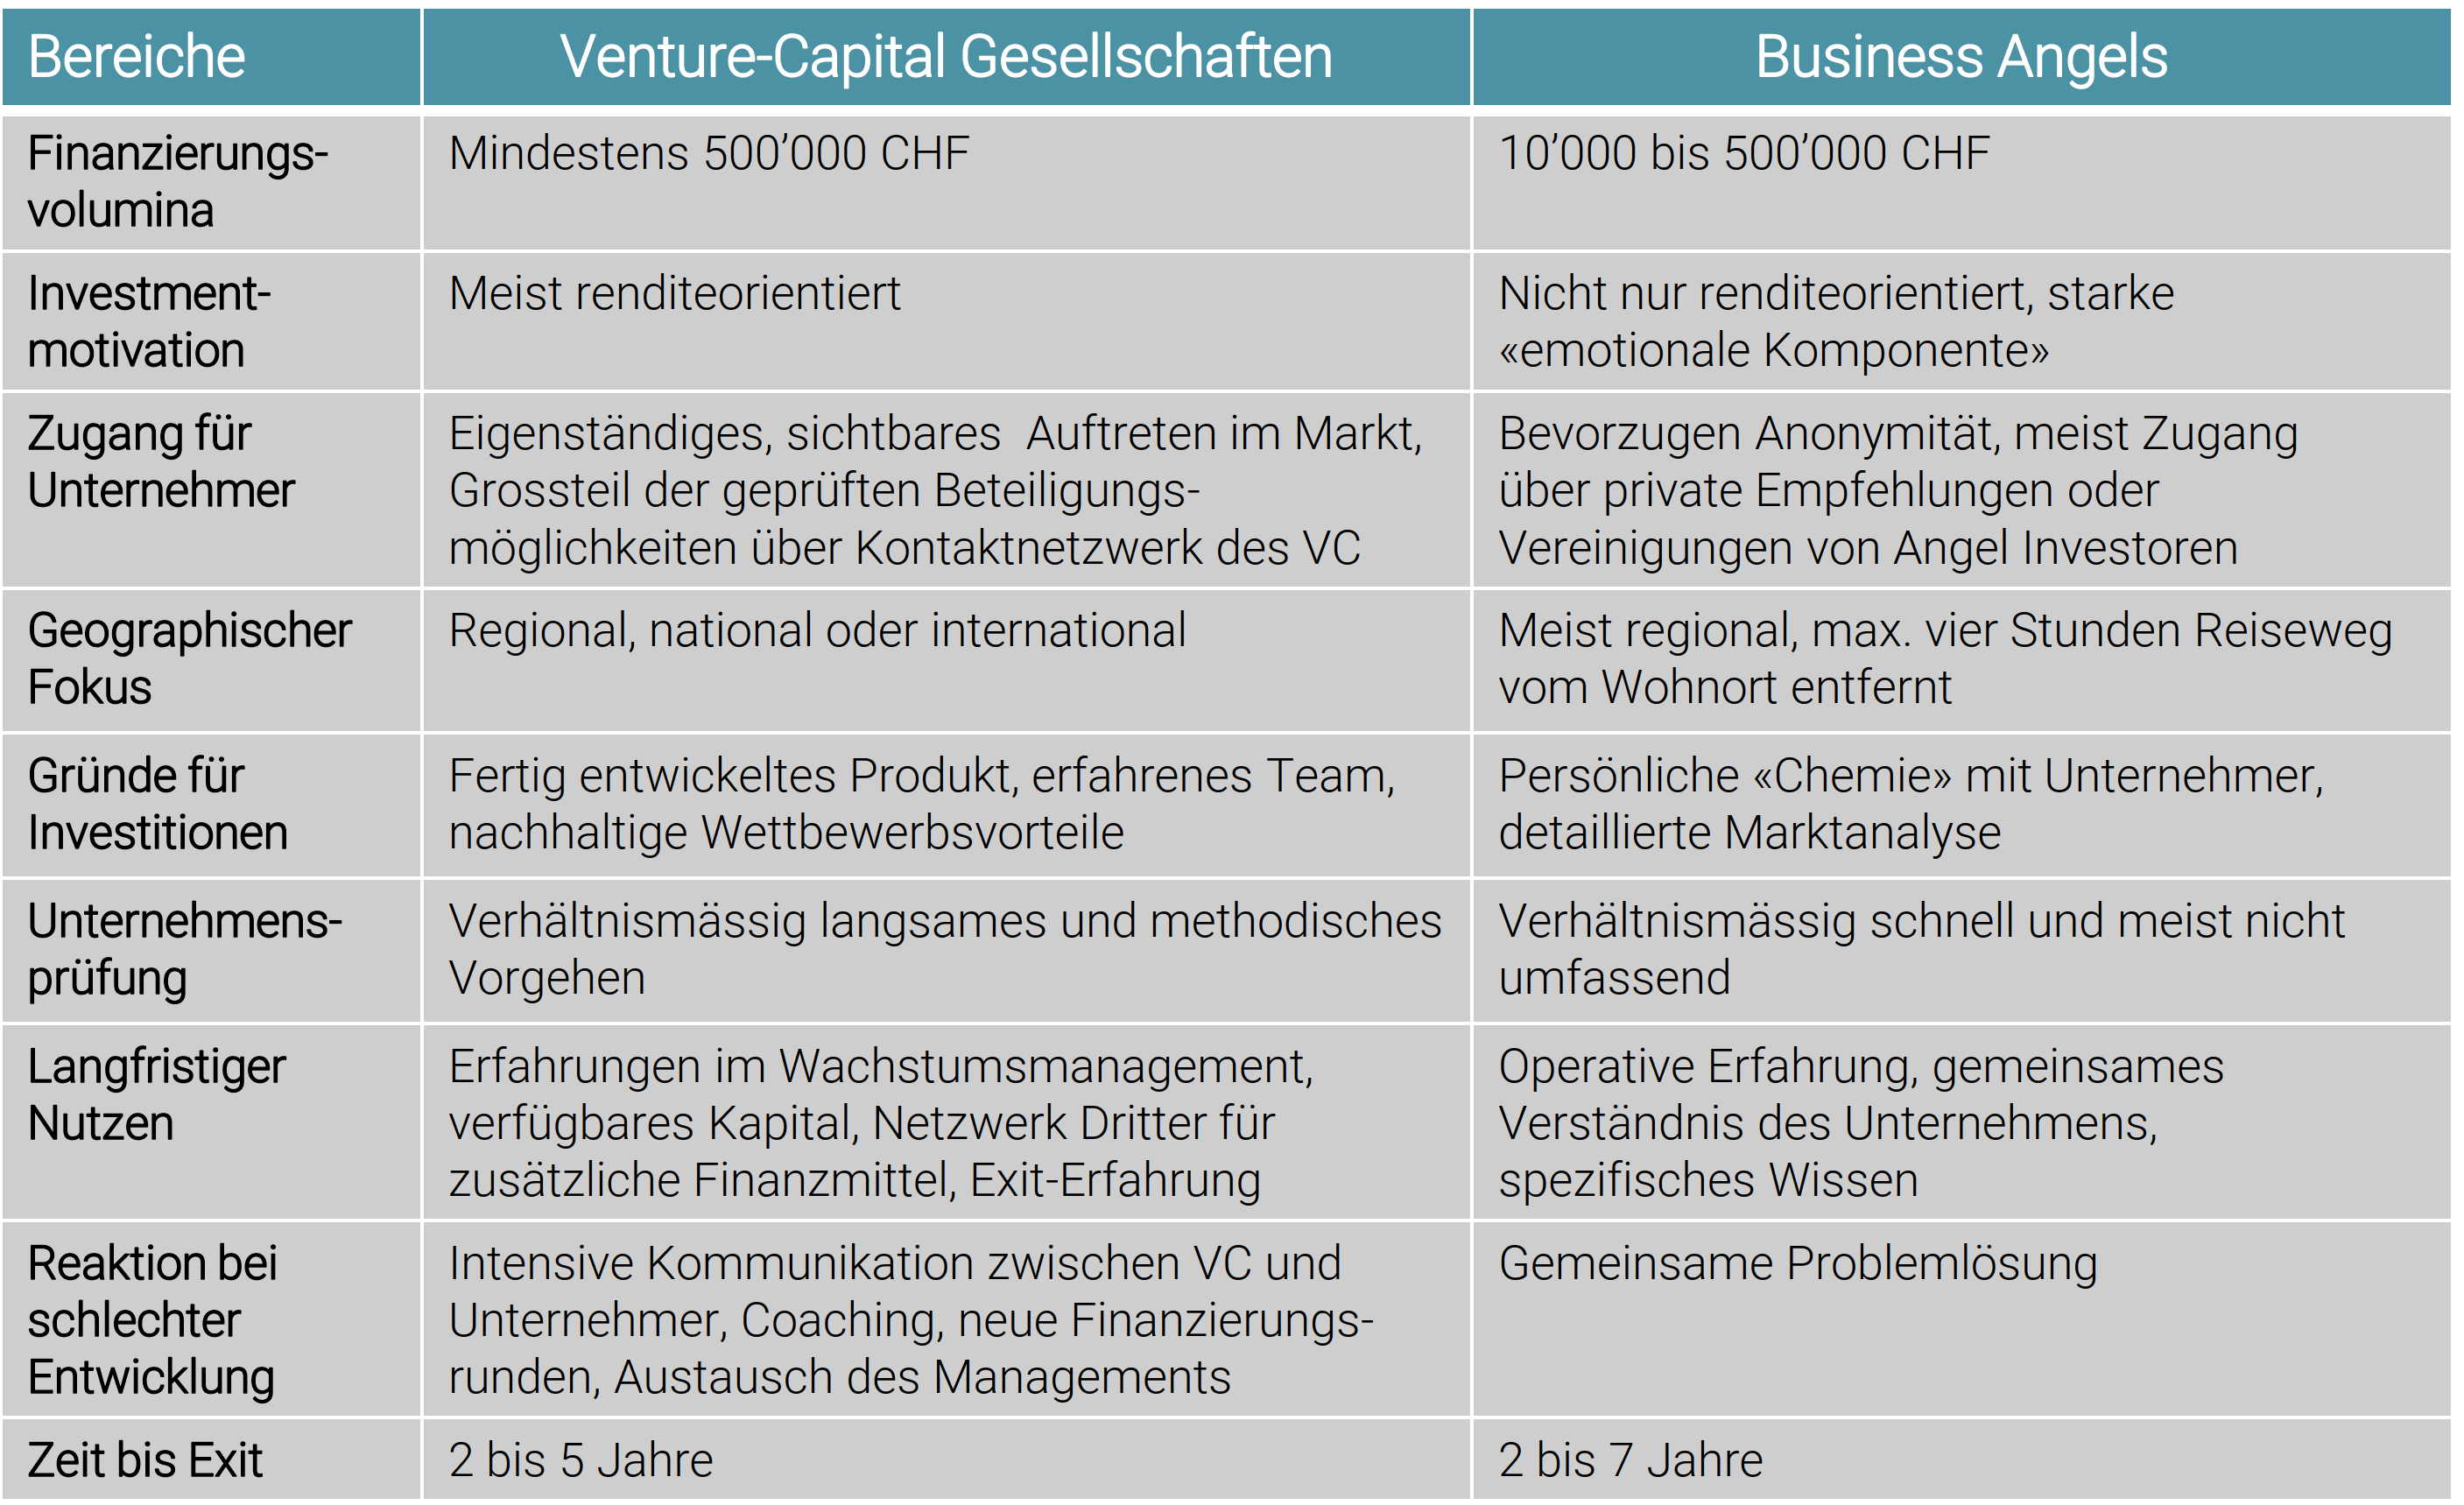
\includegraphics[width=1\linewidth]{images/vc_vs_ba}